
\onecolumn
\chapter{Office 365 の設定}
\label{chap:O365設定1}


第\ref{chap:O365設定1}章では、Windows デバイスの展開に必要な Office 365 の設定に関して解説いたします。\ref{sec:メールドメインの追加}項では、教育機関が所有するメールドメインの追加方法に関して解説し、\ref{sec:ユーザー登録}項では、Office 365 へのユーザーアカウントの追加に関して解説いたします。 
  
%%%%%%%%%%%%%%%%%%%%%%%%%%%%%%%%%%%%%%%%%%%%%%%%%%%%%%%%%%%%%%%%%%%%%%%%%%%%%%%%
\begin{figure*}[htbp]
    \section{Microsoft 365 管理センターにアクセスする}
    \label{sec:M365管理センター}
\end{figure*}
%%%%%%%%%%%%%%%%%%%%%%%%%%%%%%%%%%%%%%%%%%%%%%%%%%%%%%%%%%%%%%%%%%%%%%%%%%%%%%%%

\begin{figure*}[h]
    \begin{minipage}{0.6\textwidth}
        \vspace{-2cm}
        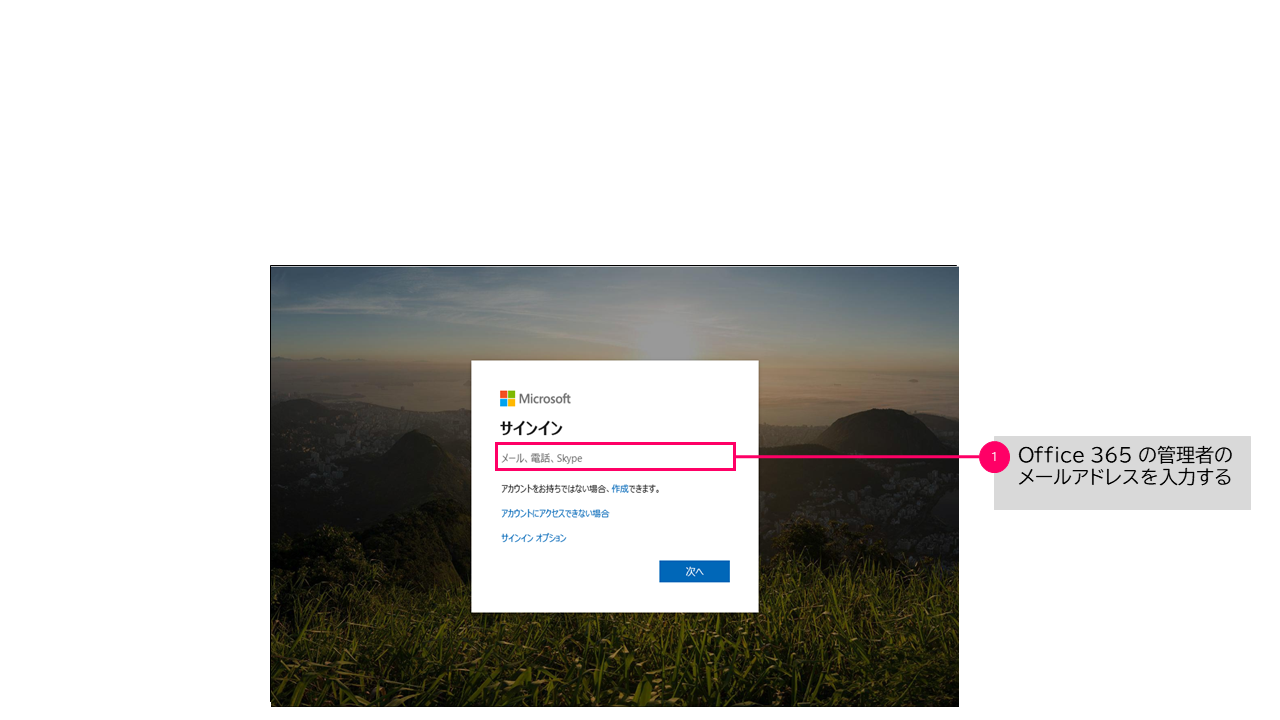
\includegraphics[width=10cm]{figures/M365_setting1-00.png}
    \end{minipage}
    \begin{minipage}{0.4\textwidth}
        1. Webブラウザから、\url{<https://portal.office.com/>} にアクセスします。サインインの画面が表示されたら、Office 365 の管理者のメールアドレスとパスワードでログインします。
    \end{minipage}

\end{figure*}

\begin{figure*}[h]
    \begin{minipage}{0.6\textwidth}
        \vspace{-1.5cm}
        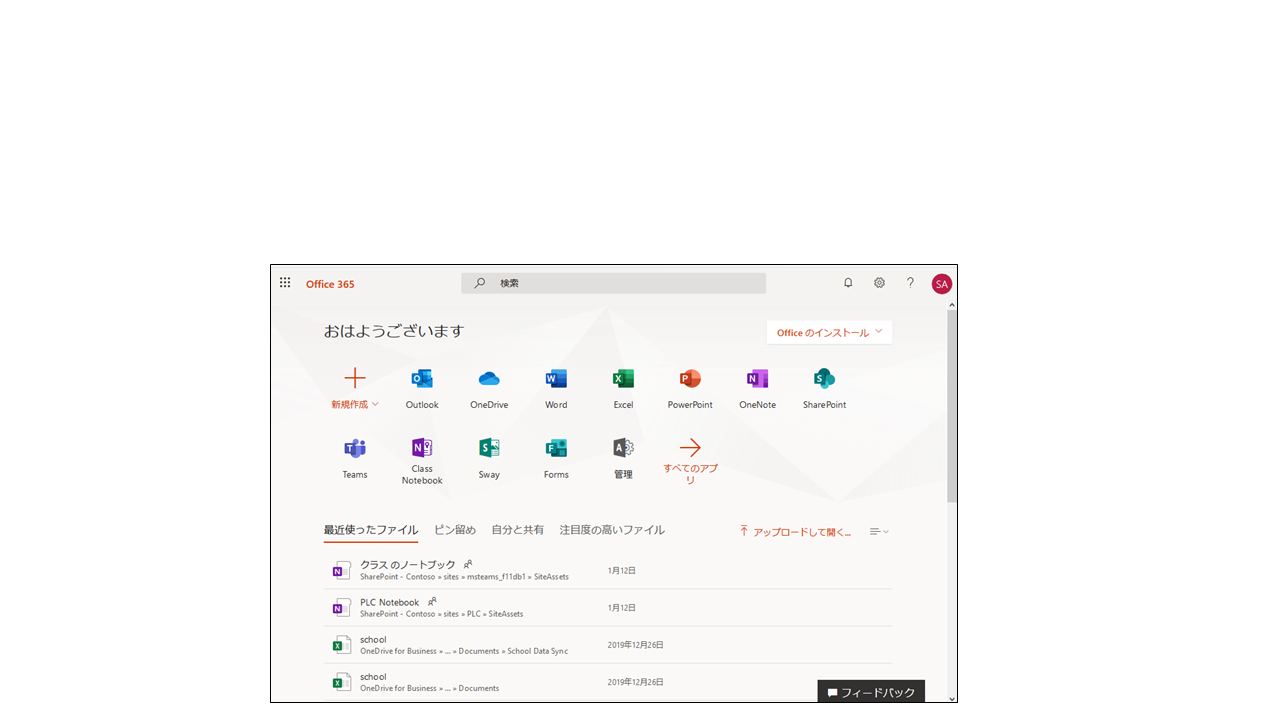
\includegraphics[width=10cm]{figures/M365_setting1-01.png}
    \end{minipage}
    \begin{minipage}{0.4\textwidth}
        2. ログインが完了すると Microsoft 365 の管理画面が表示されます。
    \end{minipage}
    \vspace{4cm}
\end{figure*}

%%%%%%%%%%%%%%%%%%%%%%%%%%%%%%%%%%%%%%%%%%%%%%%%%%%%%%%%%%%%%%%%%%%%%%%%%%%%%%%%
\begin{figure*}[h]
    \section{メールドメインの追加}
    \label{sec:メールドメインの追加}
\end{figure*}
%%%%%%%%%%%%%%%%%%%%%%%%%%%%%%%%%%%%%%%%%%%%%%%%%%%%%%%%%%%%%%%%%%%%%%%%%%%%%%%%

\begin{figure*}[h]
    \begin{minipage}{0.6\textwidth}
        \vspace{-1.0cm}
        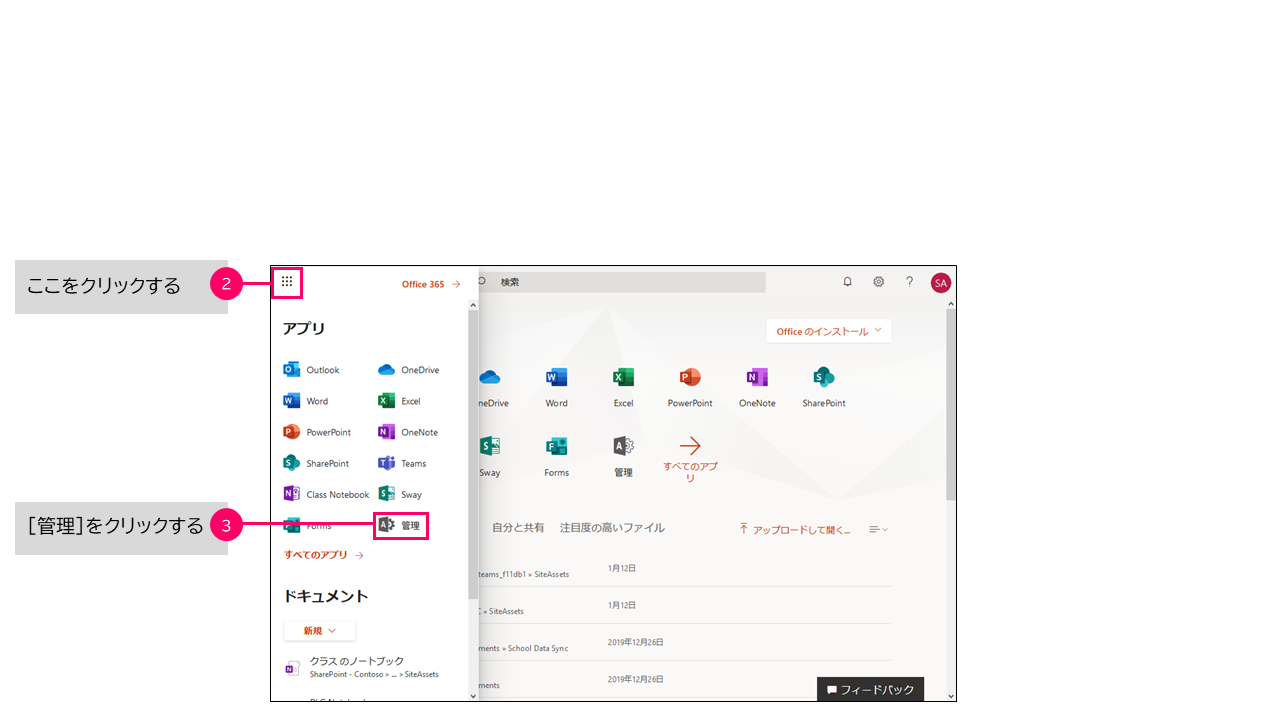
\includegraphics[width=10cm]{figures/M365_setting1-02.png}
    \end{minipage}
    \begin{minipage}{0.4\textwidth}
        3. 画面右上のメニューアイコンをクリックしてください。\\
        4. \textbf{【管理】}をクリックしてください。
    \end{minipage}
\end{figure*}

\begin{figure*}[h]
    \begin{minipage}{0.6\textwidth}
        \vspace{-2.1cm}
        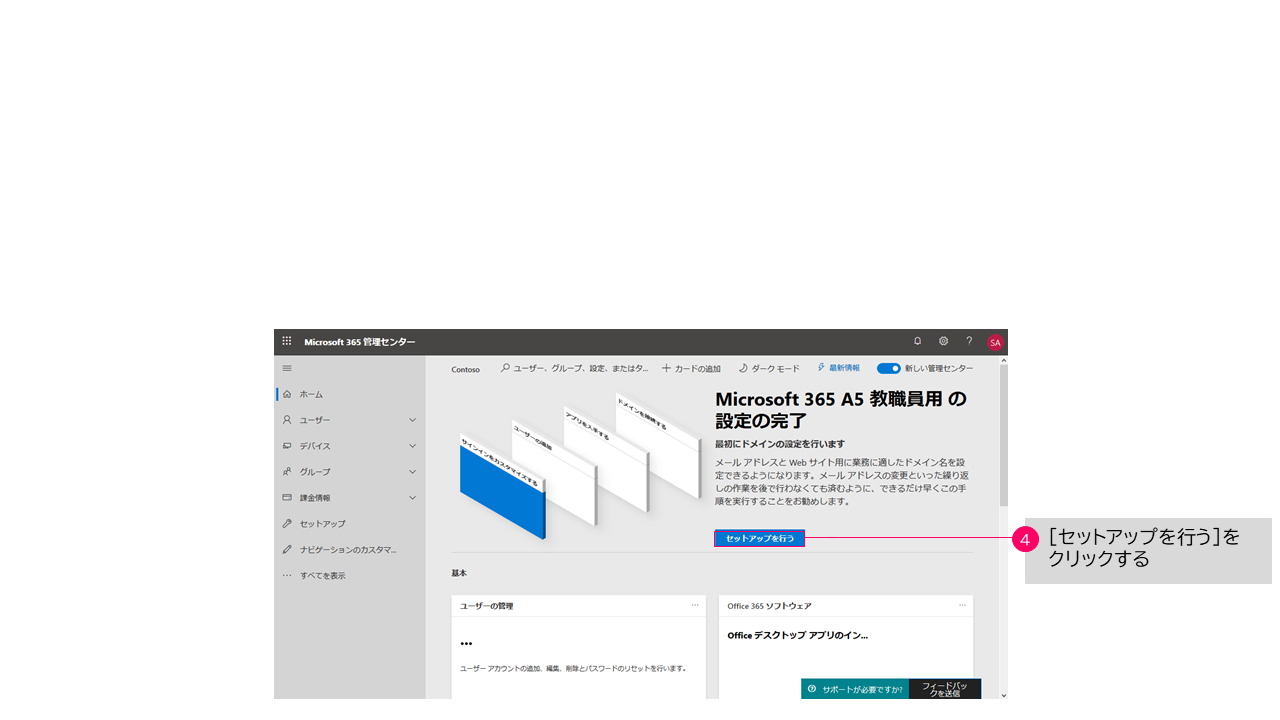
\includegraphics[width=10cm]{figures/M365_setting1-03.png}
    \end{minipage}
    \begin{minipage}{0.4\textwidth}
        5. \textbf{【セットアップを行う】}をクリックしてください。
    \end{minipage}
\end{figure*}

\begin{figure*}[htbp]
    \begin{minipage}{0.6\textwidth}
        \vspace{-2cm}
        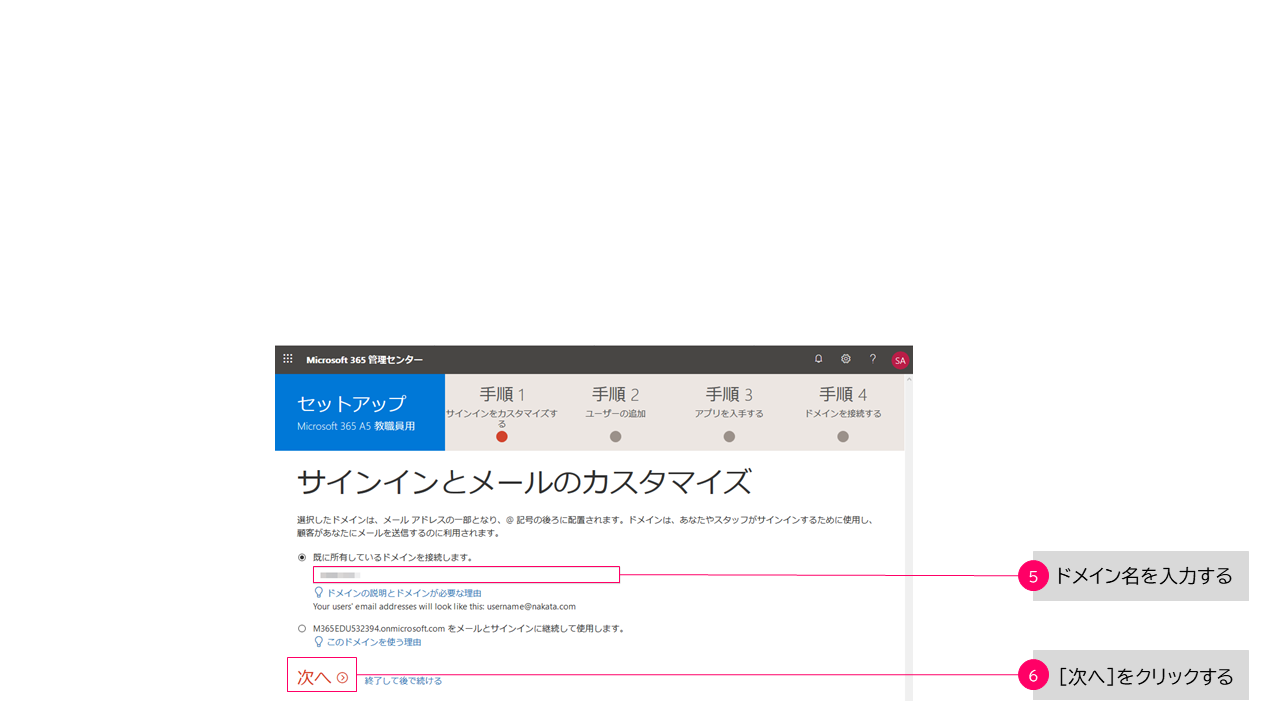
\includegraphics[width=10cm]{figures/M365_setting1-04.png}
    \end{minipage}
    \begin{minipage}{0.4\textwidth}
        6. \textbf{「サインインとメールのカスタマイズ」}の画面が表示されたら、所有しているメールドメインを入力し、\textbf{【次へ】}をクリックしてくださだい。
    \end{minipage}
    \vspace{0.5cm}
\end{figure*}

\begin{figure*}[htbp]
    \begin{minipage}{0.6\textwidth}
        \vspace{-1.5cm}\hspace{-0.5cm}
        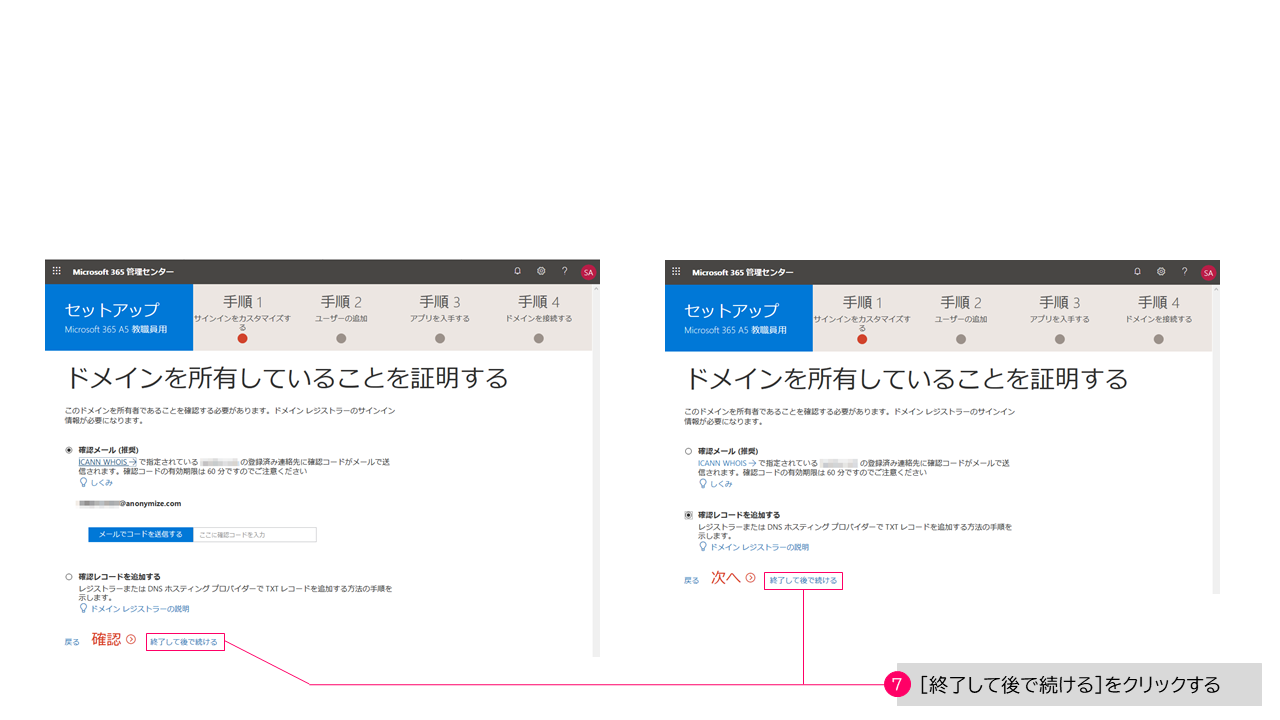
\includegraphics[width=10cm]{figures/M365_setting1-05.png}
    \end{minipage}
    \begin{minipage}{0.4\textwidth}
        7. \textbf{ドメインを所有していることを証明する】}の画面が表示されます。ドメインの所有権の証明する方法としては (1) ICANN WHOS \url{<https://lookup.icann.org/>} に登録しているメールアドレスに確認コードを送り、その確認コードで証明する方法と (2) DNSにTXTレコードを追加し証明する方法の2種類があります。どちらかの方法でドメインの所有権を証明しましたら、\textbf{【終了して後を続ける】}をクリックしてください。
    \end{minipage}
\end{figure*}



%%%%%%%%%%%%%%%%%%%%%%%%%%%%%%%%%%%%%%%%%%%%%%%%%%%%%%%%%%%%%%%%%%%%%%%%%%%%%%%%
\begin{figure}[htbp]
    \section{ユーザー登録}
    \label{sec:ユーザー登録}

    \hspace{8pt} Windows デバイスを Intune for Education で管理するためには、Windows デバイスを利用するユーザーをあらかじめOffice 365に登録しておく必要があります。
    Office 365 にユーザーを登録する方法としては、Microsoft 365 管理センターから GUI(Graphical User Interface) で1人1人登録する方法がありますが、ここでは CSVファイルを使用して一括登録する方法を解説します。\\
\end{figure}
%%%%%%%%%%%%%%%%%%%%%%%%%%%%%%%%%%%%%%%%%%%%%%%%%%%%%%%%%%%%%%%%%%%%%%%%%%%%%%%%



%%%%%%%%%%%%%%%%%%%%%%%%%%%%%%%%%%%%%%%%%%%%%%%%%%%%%%%%%%%%%%%%%%%%%%%%%%%%%%%%
\begin{figure}[]
    \subsection{Azure Active Direcoty のユーザーの属性情報}

    \hspace{8pt} Office 365 のアカウント管理を行っている Azure Active Directory には、ログインID(メールアドレス)[必須]、表示名[必須]、姓、名以外にもユーザーに紐づく様々な属性情報を持つことができます。

    \hspace{8pt} Office 365 の特徴のひとつにユーザーの属性情報を使用してあるグループに動的にユーザーを追加、削除する「\textbf{動的グループ}」というものがあります。この動的グループを使って、Teams へのユーザーの追加・削除や Intune で管理するデバイスの設定をグループごとに設定することができますので、グループへのユーザ―の追加と削除に必要な管理費用を大幅に削減することが可能です。動的グループを利用することで、年次更新で児童・生徒の学年を変更するだけで、Windows デバイスで使用するアプリケーションを変更したり、教員が学校を移動した際に、移動先の学校が所有するSharepoint上のファイルサーバーに自動的にアクセスできるようにするなどのことが実現できるようになります。

    \hspace{8pt} 動的グループを利用することで、グループの管理に係る管理コストを大幅に削減できますので、動的グループを利用できるように Azure Active Directory にユーザーの属性情報を登録することを強くお勧めします。
\end{figure}
\vspace{6cm}
%%%%%%%%%%%%%%%%%%%%%%%%%%%%%%%%%%%%%%%%%%%%%%%%%%%%%%%%%%%%%%%%%%%%%%%%%%%%%%%%




%%%%%%%%%%%%%%%%%%%%%%%%%%%%%%%%%%%%%%%%%%%%%%%%%%%%%%%%%%%%%%%%%%%%%%%%%%%%%%%%
\begin{figure}[]
    \subsection{GIGAスクールで定義するユーザーの属性情報}

    \hspace{8pt} ではGIGAスクール構想では、ユーザーにどのような属性情報を持たせればよいのでしょうか。表\ref{tab:AAD属性値}は一例になります。各教育機関毎にどのような属性値をユーザーに持たせればよいのか検討してください。
\end{figure}
%%%%%%%%%%%%%%%%%%%%%%%%%%%%%%%%%%%%%%%%%%%%%%%%%%%%%%%%%%%%%%%%%%%%%%%%%%%%%%%%


\begin{table*}[hp]
    \caption{GIGAスクール構想における Azure AD の属性値}
    \label{tab:AAD属性値}
    \scalebox{0.9}{
    \begin{tabular}{llll}
        \hline\hline
        Azure ADの属性名 & 表示名の名前 & GIGAスクールでの属性値 & 備考 \\
        \hline
        userPrincipalName (必須)& ユーザー名 & ユーザー名 & Office 365 にログインするためのユーザー名 \\
        \hline
        DisplayName (必須)& 名前 & 名前 & Office 365のサービス内で表示されるもの \\
        \hline
        givenName & 名 & 名 & \\
        \hline
        surName & 姓 & 姓 & \\
        \hline
        userType & ユーザータイプ & 在学中:Member & \\
        &  & 卒業・離職: Other& \\
        \hline
        jobTitle & 役職 & 児童・生徒:studnet & \\
        & & 職員:staff & \\
        & & 教員:teacher & \\
        \hline
        department & 部署 & 学校名 & \\
        \hline
        officeLocation & 会社 & 学年 & \\
        \hline
        businessPhone & 電話番号 & クラス名 & \\
        \hline
        streetAddress & 番地 & 担当科目 & 教員の場合のみ入力\\
        \hline
        city & 市区町村 & 教育委員会名 & \\
        \hline
        state & 都道府県 & 都道府県 & \\
        \hline
        country & 国 & 国 & \\
        \hline \hline
    \end{tabular}
    }
\end{table*}


%%%%%%%%%%%%%%%%%%%%%%%%%%%%%%%%%%%%%%%%%%%%%%%%%%%%%%%%%%%%%%%%%%%%%%%%%%%%%%%%
\begin{figure}[h]
    \subsection{ユーザー一括登録用のCSVファイルの準備}

    \hspace{8pt} Office 365 のユーザーをCSV形式のファイルで登録するためには、まず初めにCSV形式\footnote{CSV形式とは、カンマ(,)で区切られた値を含む形式です。}のファイルのサンプルを入手する必要があります。

    \hspace{8pt} CSV形式のサンプルファイルは以下のURLよりダウンロードすることができます。

    \hspace{24pt} \url{https://www.microsoft.com/download/details.aspx?id=45485 }

    \hspace{8pt} CSV形式のファイルをダウンロードできたら、Excel でこのファイルを開きます。
\end{figure}
%%%%%%%%%%%%%%%%%%%%%%%%%%%%%%%%%%%%%%%%%%%%%%%%%%%%%%%%%%%%%%%%%%%%%%%%%%%%%%%%



\begin{figure*}[h]
    \begin{minipage}{0.6\textwidth}
        \vspace{-0.5cm}
        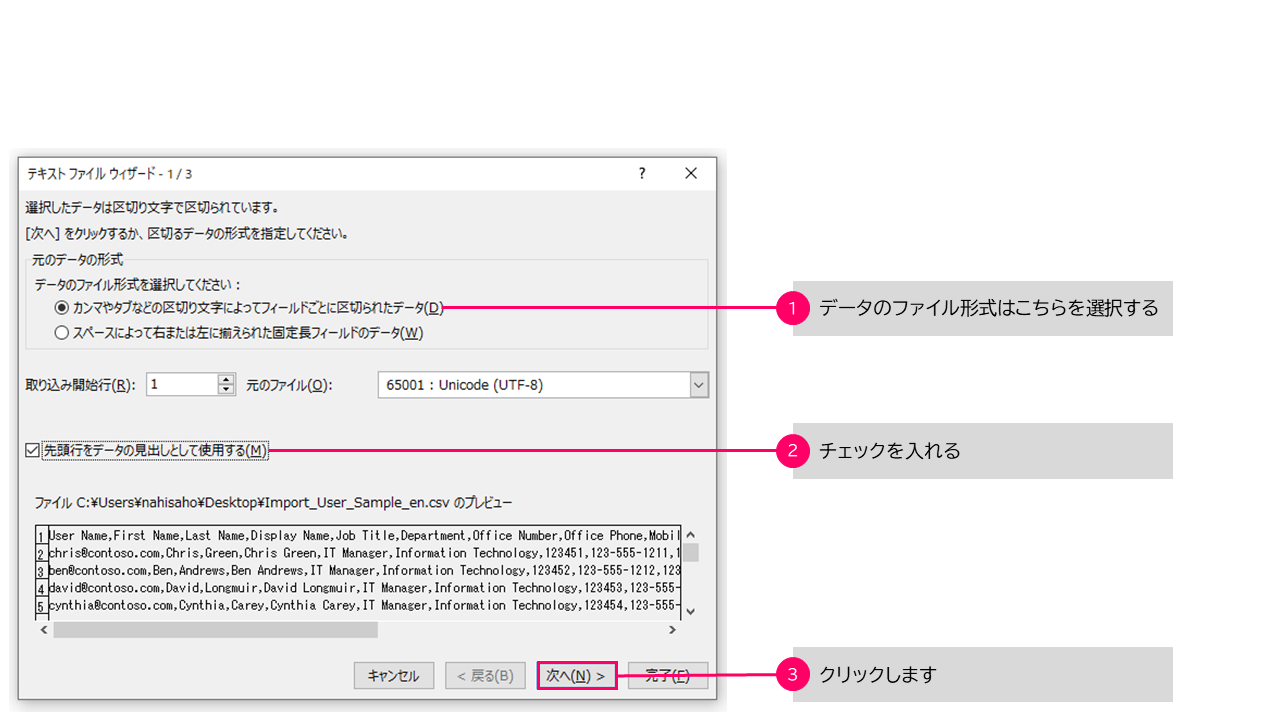
\includegraphics[width=10cm]{figures/CSV_Import-1.png}
    \end{minipage}
    \begin{minipage}{0.4\textwidth}
        \textbf{「テキストファイルウィザード 1/3」}の画面が開いたら、データのファイル形式は\textbf{【カンマやタブなどの区切り文字によってフィールドごとに区切られたデータ(D)】} を選択し、\textbf{【先頭行をデータの見出しとして使用する(M)】}にチェックを入れた後、\textbf{【次へ(N)】}ボタンをクリックしてください。
    \end{minipage}
\end{figure*}

\begin{figure*}[h]
    \begin{minipage}{0.6\textwidth}
        \vspace{-1cm}
        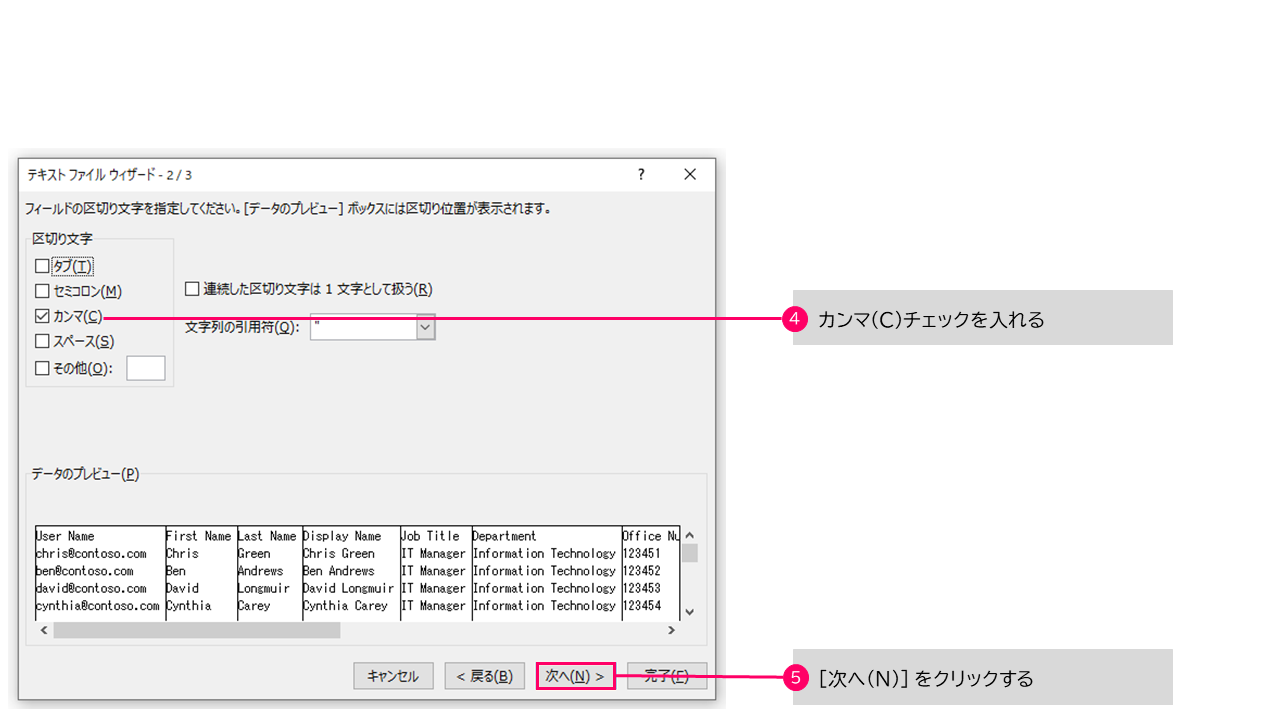
\includegraphics[width=10cm]{figures/CSV_Import-2.png}
    \end{minipage}
    \begin{minipage}{0.4\textwidth}
        \textbf{「テキストファイルウィザード 2/3」}の画面が開いたら、区切り文字は\textbf{【カンマ(C)】}にチェックをいれ、\textbf{【次へ(N)】}ボタンをクリックしてください。
    \end{minipage}
\end{figure*}

\begin{figure*}[h]
    \begin{minipage}{0.6\textwidth}
        \vspace{-1cm}
        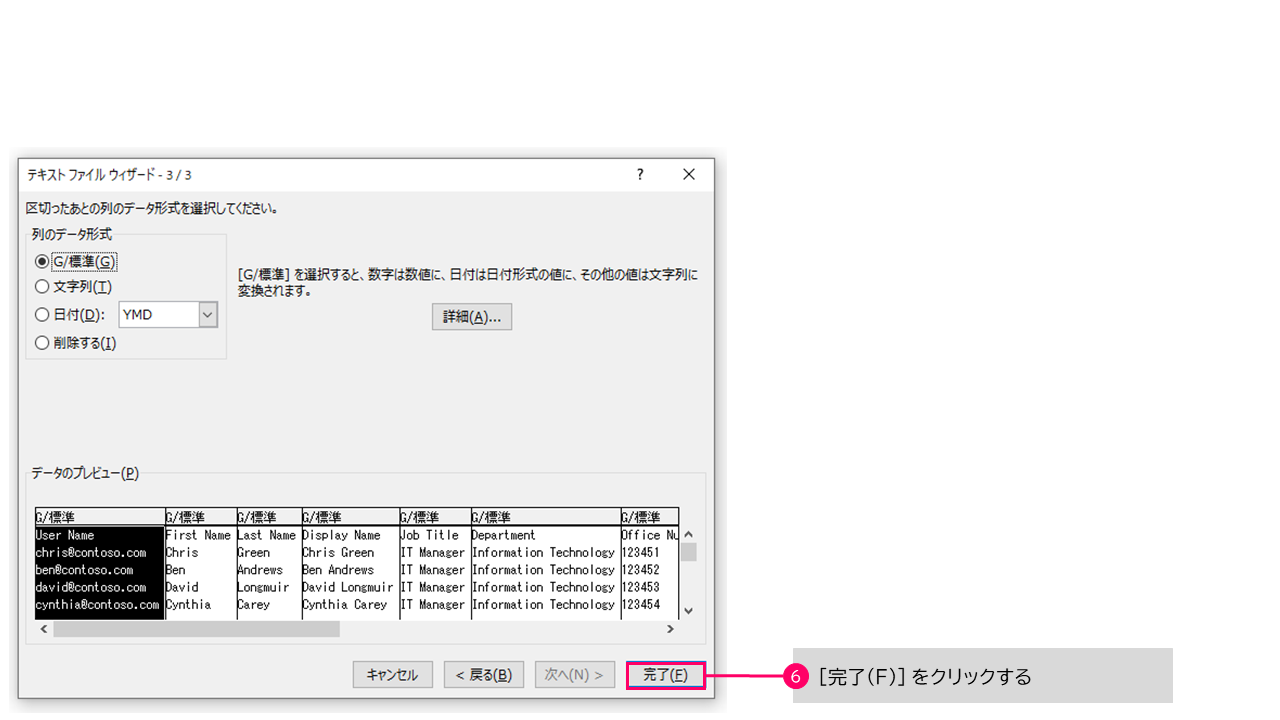
\includegraphics[width=10cm]{figures/CSV_Import-3.png}
    \end{minipage}
    \begin{minipage}{0.4\textwidth}
        \textbf{「テキストファイルウィザード 3/3」}の画面が開いたら、列のデータ形式はすべて\textbf{【G/標準】}を選択し、完了したら\textbf{【完了(F)】}をクリックしてくださだい。
    \end{minipage}
\end{figure*}

\begin{figure*}[h]
    \begin{minipage}{0.6\textwidth}
        \vspace{-2cm}
        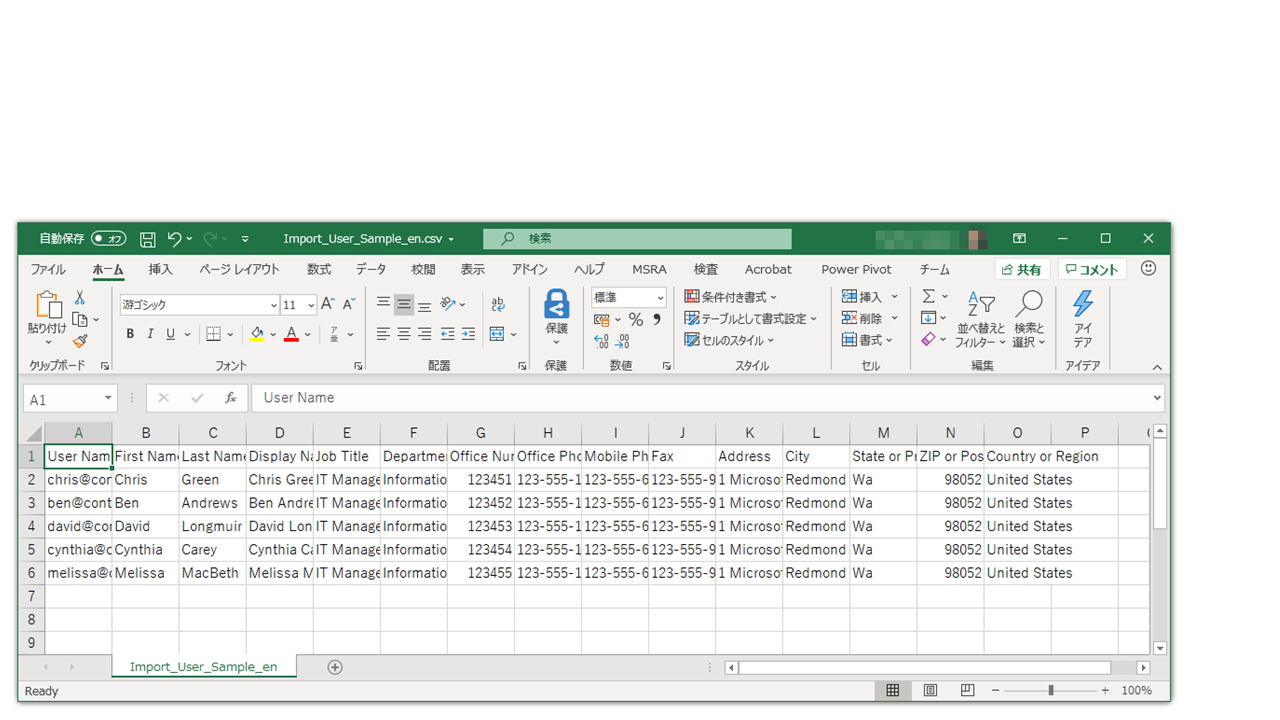
\includegraphics[width=10cm]{figures/CSV_Import-4.png}
    \end{minipage}
    \begin{minipage}{0.4\textwidth}
        Excel が開き、サンプルデータが表示されます。ユーザー登録するためのデータを入力し、CSV形式でファイルを保存してください。
    \end{minipage}

\end{figure*}

\newpage

%%%%%%%%%%%%%%%%%%%%%%%%%%%%%%%%%%%%%%%%%%%%%%%%%%%%%%%%%%%%%%%%%%%%%%%%%%%%%
\begin{figure}[]
    \subsection{CSV形式のファイルによるユーザーの一括登録}
\end{figure}
%%%%%%%%%%%%%%%%%%%%%%%%%%%%%%%%%%%%%%%%%%%%%%%%%%%%%%%%%%%%%%%%%%%%%%%%%%%%%

\begin{figure*}[h]
    \begin{minipage}{0.6\textwidth}
        \vspace{-1cm}
        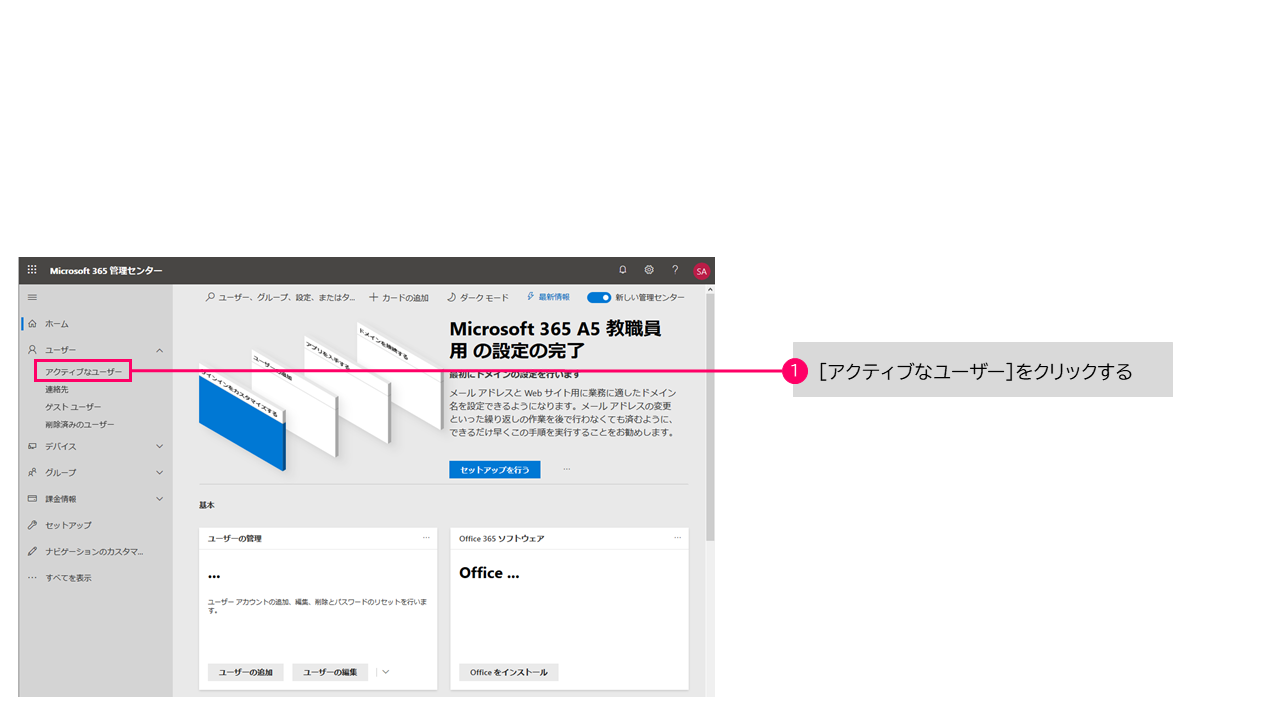
\includegraphics[width=10cm]{figures/CSV_Import-5.png}
    \end{minipage}
    \begin{minipage}{0.4\textwidth}
        Microsft 365 管理センターから\textbf{【ユーザー】→【アクティブなユーザー】}をクリックします。
    \end{minipage}
\end{figure*}

\begin{figure*}[h]
    \begin{minipage}{0.6\textwidth}
        \vspace{-1cm}
        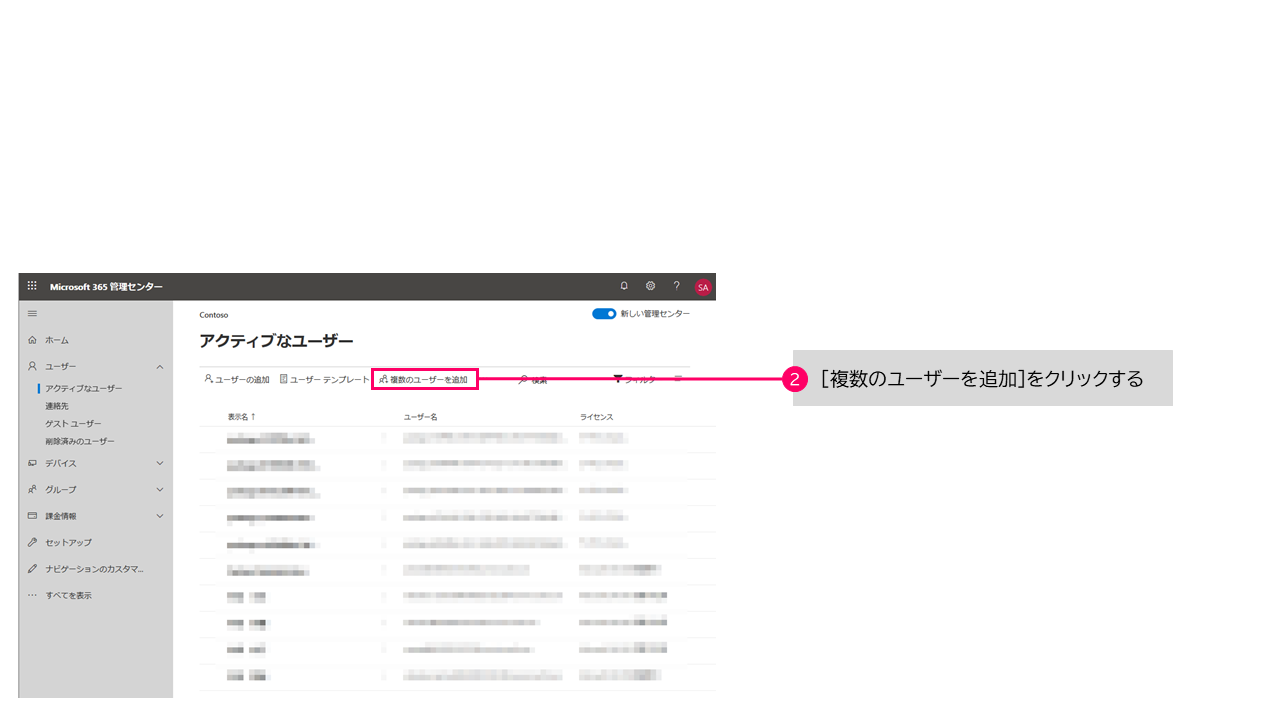
\includegraphics[width=10cm]{figures/CSV_Import-6.png}
    \end{minipage}
    \begin{minipage}{0.4\textwidth}
        \textbf{【複数のユーザーを追加】}をクリックします。
    \end{minipage}
\end{figure*}

\begin{figure*}[h]
    \begin{minipage}{0.6\textwidth}
        \vspace{-1cm}
        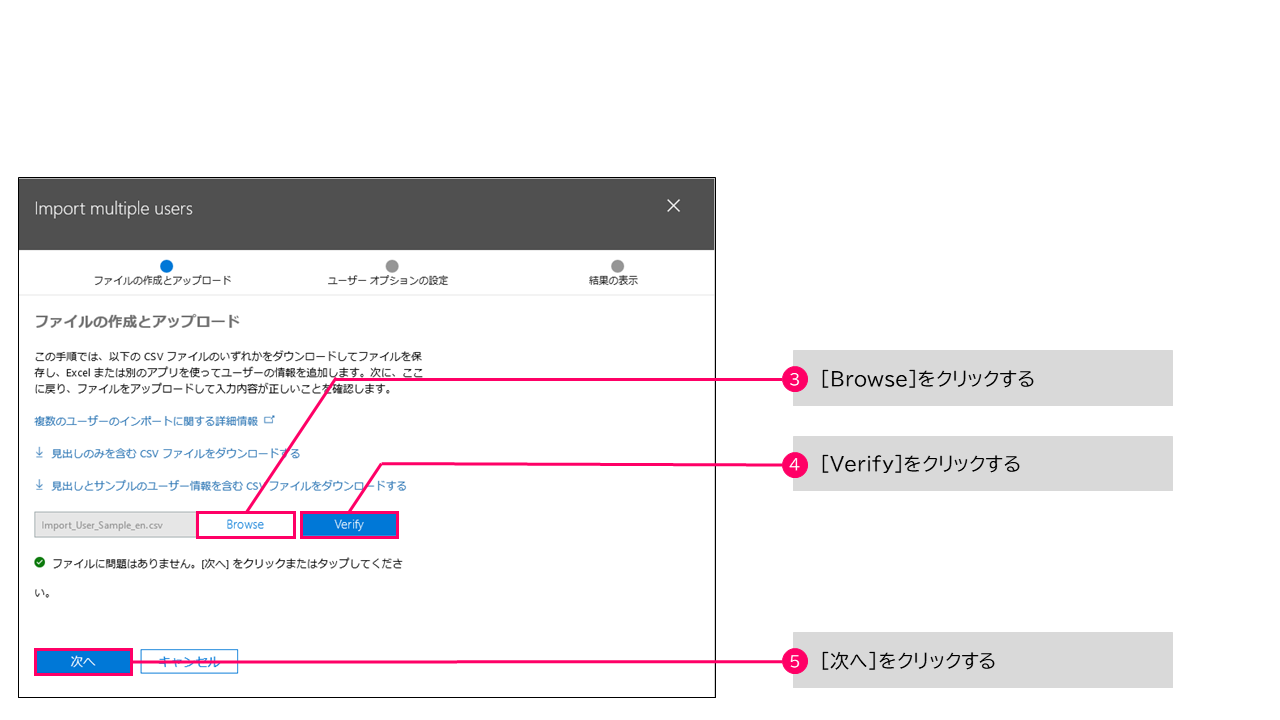
\includegraphics[width=10cm]{figures/CSV_Import-7.png}
    \end{minipage}
    \begin{minipage}{0.4\textwidth}
        \textbf{【Brows】}をクリックします。ファイルを選択する画面が表示されたら、アップロードするファイルを選んでください。\\
        ファイルがアップロードできたら\textbf{【Verify】}をクリックし、アップロードしたファイルの整合性をチェックします。\\
        アップロードしたファイルの整合性のチェックが完了したら、\textbf{【次へ】}をクリックしてください。
    \end{minipage}
\end{figure*}

\begin{figure*}[h]
    \begin{minipage}{0.6\textwidth}
        \vspace{0cm}
        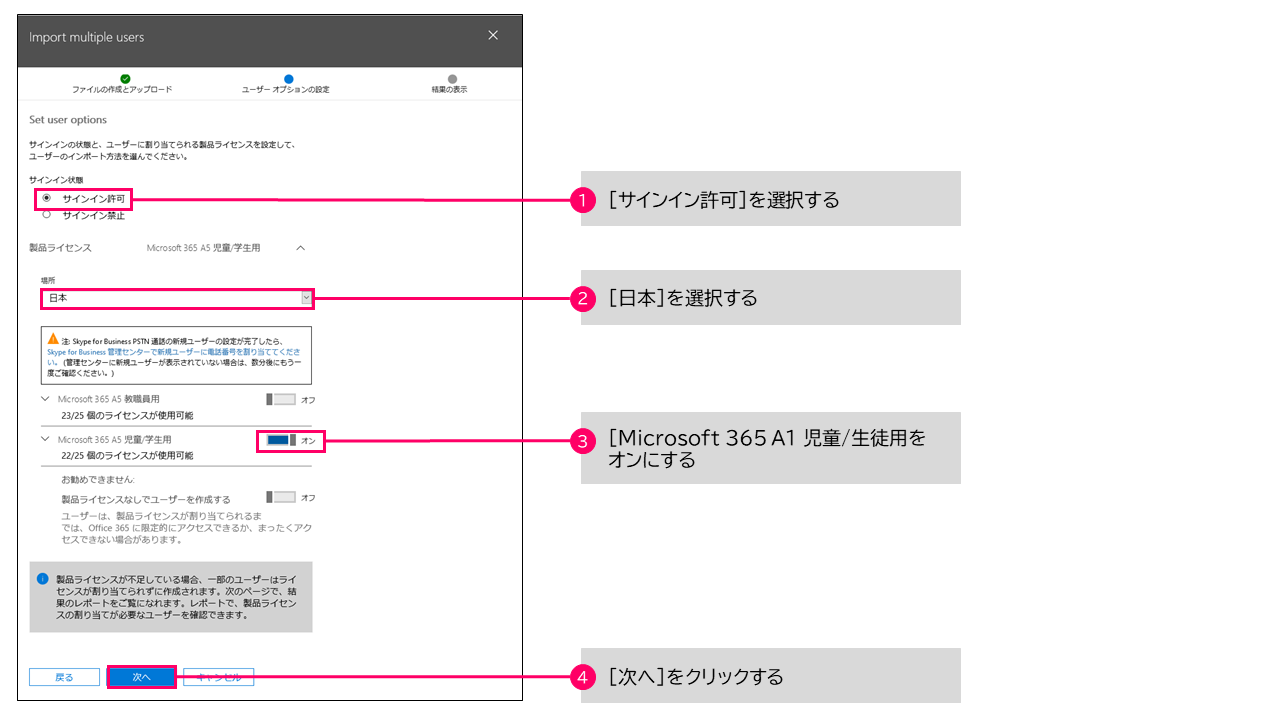
\includegraphics[width=10cm]{figures/CSV_Import-8.png}
    \end{minipage}
    \begin{minipage}{0.4\textwidth}
        サインイン状態は\textbf{【サインイン許可】}を選択します。\\
        場所は\textbf{【日本】}を選択します。\\
        ユーザーにあったライセンスを\textbf{【オン】}にしてください。\\
        すべての設定が完了したら\textbf{【次へ】}をクリックしてください。
    \end{minipage}
\end{figure*}

\begin{figure*}[h]
    \begin{minipage}{0.6\textwidth}
        \vspace{-1cm}
        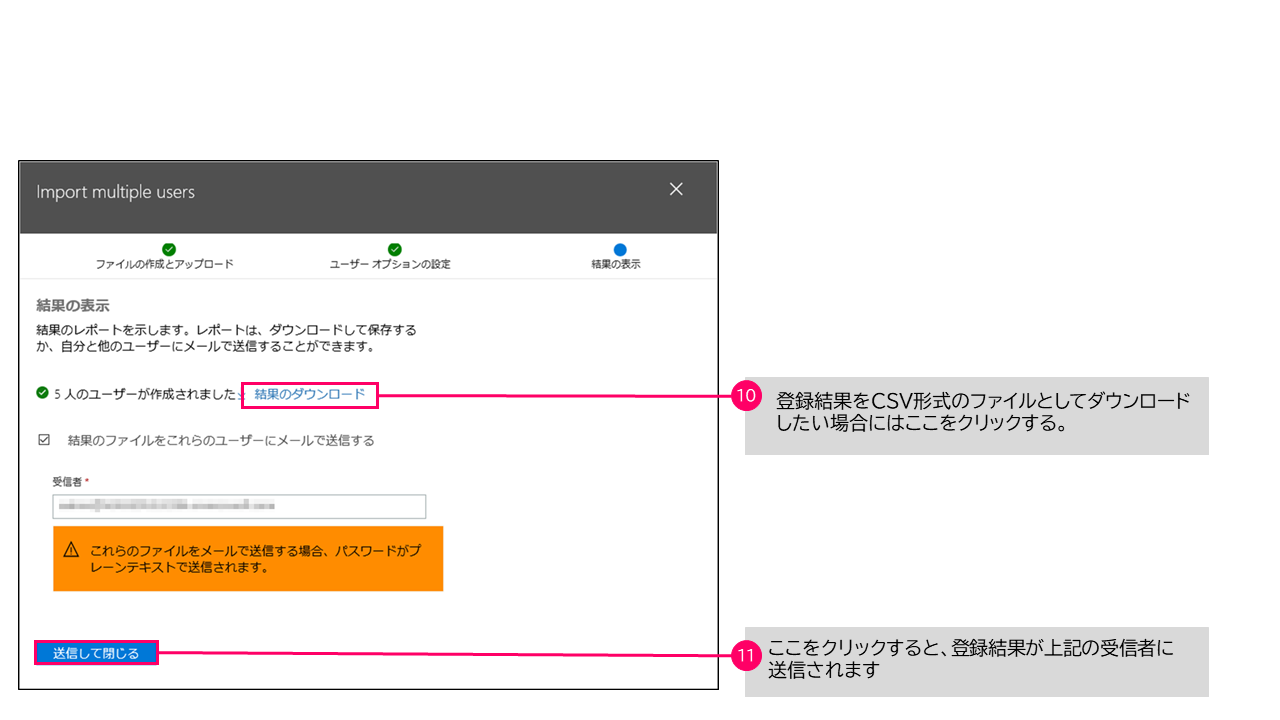
\includegraphics[width=10cm]{figures/CSV_Import-9.png}
    \end{minipage}
    \begin{minipage}{0.4\textwidth}
        ユーザー登録が完了すると\textbf{「結果の表示」}の画面が表示されます。登録結果をCSV形式のファイルでダウンロードしたい場合には、\textbf{【結果のダウンロード】}をクリックしてください。\\
        \textbf{【送信して閉じる】}をクリックすると、登録結果が上記の受信者に送信されます。
    \end{minipage}
    \vspace{17cm}
\end{figure*}

